\section{Nomenclature}

The first two sections of the introduction examine the organization of biomedical knowledge, and several of the challenges faced during the process.
These challenges span from unifying the nomenclature of biologically relevant entities used in the published biomedical literature to extracting the biological knowledge and context surrounding those entities.

\subsection{Issues with Gene Nomenclature}

The nomenclature of genes and gene products is a particularly egregious example of poor nomenclature within the biomedical domain.
Genes often have several names as well as several incomprehensible acronyms, or gene symbols.
For example, the \ac{HGNC}~\cite{Yates2017} and Entrez Gene~\cite{Maglott2011} database list that the human gene microtubule associated protein tau (hgnc:HGNC:6893, ncbigene:4137) has previously been named the G protein
$\beta1$/$\gamma2$ subunit-interacting factor 1 and the protein phosphatase 1,
regulatory subunit 103.
Like with many genes, it is often acronymized to MAPT in text, but it has additionally been previously referenced with DDPAC, FLJ31424, FTDP-17, MAPTL, MGC13854, MTBT1, MTBT2, MSTD, PPND, and PPP1R103.

Neither genes' names nor their gene symbols convey their host species, which leads to further ambiguities in articles discussing orthologs in model organisms.
The organization responsible for mouse gene nomenclature, \ac{MGI}~\cite{Blake2017}, names the mouse orthologous gene as microtubule-associated protein tau (mgi:MGI:97180, ncbigene:17762) and lists the gene symbol as Mapt.
In this example, the name varies from the human ortholog with the introduction of a hyphen between "microtubule" and "associated."
The gene symbol differs only in capitalization.
Similarly, the organization for rat genome nomenclature, the \ac{RGD}~\cite{Shimoyama2015}, names the rat orthologous gene as microtubule-associated protein tau (rgd:69329; ncbigene:29477)---exactly as in \ac{MGI}.
While these orthologs from common model organisms have had related names, organisms with genetic drift such as Zebrafish have several orthologs named microtubule-associated protein tau a (zfin:ZDB-GENE-081027-1) and microtubule-associated protein tau b (zfin:ZDB-GENE-081027-2) whose gene symbols are listed as mapta and maptb, respectively.
Other orthologs to human microtubule-associated protein tau can be found in Homologene (homologene:74962), Ensembl~\cite{Zerbino2018}, \ac{HGNC}, \ac{MGI}, PomBase, \ac{RGD}, Xenbase, and \ac{ZFIN}.
The \ac{HCOP}~\cite{Wright2005} aggregates these and several other sources of curated and predicted orthologies.

\subsection{Nomenclature Consortia of Genes and Proteins}

Most biologically relevant named entities have many names.
For example, many genes were independently discovered and characterized in different labs and therefore named differently.
As resources for exchanging genomic and protein sequences have become more ubiquitous in the last three decades since the inception of the Entrez gene database in 1991 and the \ac{HGNC} in 1996, it has become easier to reduce those duplicates.
However, this does not solve the problem of establishing a canonical name for each entity.
As stated in the previous section, several committees and consortia have formed to standardize the nomenclature used for genes for each species (Table~\ref{tab:gene_nomenclature_databases}).

\begin{table}
    \centering
    \caption{Example model organism gene nomenclature databases}
    \label{tab:gene_nomenclature_databases}
    \begin{tabular}{ l l l }
        Organism & Database & Reference \\
        \hline
        Human & \ac{HGNC} &\cite{Yates2017} \\
        Vertebrae & VGNC &\cite{Yates2017} \\
        Mouse & MGI &\cite{Blake2017} \\
        Rat & RGD &\cite{Shimoyama2015} \\
        Zebrafish & ZFIN &\cite{Howe2013}  \\
        Drosophila (fly) & FlyBase &\cite{Thurmond2019}\\
        Xenopus (frog) & Xenbase &\cite{Karimi2018}  \\
        Yeast & SGD &\cite{Cherry2012} \\
        - & Entrez Gene &\cite{Maglott2011}  \\
    \end{tabular}
\end{table}

\subsection{Nomenclature Consortia of Other Entities}

Besides gene nomenclature, there are several other biologically relevant physical entities and higher-order processes that have have the same issues in nomenclature.
Further, for higher-order processes like pathways, mechanisms, and biological processes, it not only remains unclear what to name each example, but where their boundaries lie.
However, deference to entities beyond genes and proteins is required to fully describe complex biology.
Thus, several groups have attempted to standardize and control the nomenclature of these entities (Table~\ref{tab:other_nomenclature_databases}).

\begin{table}
    \centering
    \caption{Example entity types of interest in the biomedical domain and corresponding nomenclature sources}
    \label{tab:other_nomenclature_databases}
    \begin{tabular}{ l l }
        Entity Type & Resources \\
        \hline
        Transcripts & Ensembl, miRBase \\
        Proteins & UniProt \\
        Protein Families & InterPro, neXtProt, FamPlex, ExPASy, Signor \\
        Protein Complexes & Complex Portal, FamPlex, Signor, Gene Ontology \\
        Biological Processes & Gene Ontology MeSH \\
        Pathways & Reactome, WikiPathways, KEGG \\
        Conditions and Phenotypes & Disease Ontology, Human Phenotype Ontology, MeSH
    \end{tabular}
\end{table}

\subsection{Practical Considerations in Named Entity Recognition}

Besides further synonyms and morphological variations, Bachman \textit{et al.}~\cite{Bachman2018} outlined several affixes corresponding to post-translational modification state, experimental context, or other categories (Table~\ref{tab:affix_categories}).

\begin{table}
    \centering
    \caption{Examples of affix categories in the FamPlex ontology adapted from Table 2 of~\cite{Bachman2018}}
    \label{tab:affix_categories}
    \begin{tabular}{ l l }
        Affix Category & Example \\
        \hline
        Experimental context & eGFP-\{Gene name\} \\
        Protein state & phospho-\{Gene name\} \\
        Inhibitor & shRNA-\{Gene name\} \\
        Generic descriptor & Proto-oncogene \{Gene name\} \\
        Species & mmu-\{Gene name\} \\
        mRNA grounding & \{Gene name\} mRNA
    \end{tabular}
\end{table}

Bachman \textit{et al.} also considered issues with recognizing proteins, protein families, and protein complexes~\cite{Bachman2018}.
The biomedical literature often references multi-protein families (e.g., RAS, AKT) and multi-subunit complexes (e.g., NF-kB, AP-1) rather than their constituent proteins.
For example, the protein family of phospholipase C enzymes, more commonly referenced as PLC, contains not only individual genes (e.g., PLCE1), but also subfamilies such as PLCG, which contains the genes PLCG1 and PLCG2.
The NF-kB complex comprises five proteins (i.e., RELA, RELB, REL, NFKB1, and NFKB2) and poses the further challenge of how named entities should be interpreted after recognition.

\subsection{Automating Named Entity Recognition}

In practice, automating the process of recognizing named entities has three major tasks: coreference resolution, \ac{NER}, and entity linking.

\subsubsection*{Coreference Resolution}

During the process of coreference resolution, antecedents or anaphors are identified and connected to their preceding or succeeding words or phrases.
In the example "The EGFR belongs to a family of protein-tyrosine kinase receptors. It is activated by the binding of EFG.", coreference resolution identifies that the subject of the second sentence, \textit{it}, refers to EGFR.
There are several classical rule-based coreference resolution algorithms including the syntax-based Hobbs theory~\cite{Hobbs1978}, discourse-based centering theory~\cite{Brennan1987}, and syntactic knowledge-based RAP algorithm~\cite{Brennan1987}.
However, recent improvements to coreference resolution have focused on four categories of machine learning techniques: mention-pair models~\cite{Soon2001,Ng2002,Bengtson2008}, entity-mention models~\cite{Luo2004,Yang2004,Yang2008}, mention-ranking models~\cite{Lee2011,Denis2007,Rahman2009,martschat2015}, and cluster-ranking models~\cite{Rahman2011,Ma2014,Clark2016}.
Recent work has focused on using recurrent neural networks with architectures such as the bi-directional long-short-term memory~\cite{Li2018} and variants such as the bi-directional long-short-term memory conditional random field~\cite{Giorgi526244}.

\subsubsection*{Named Entity Recognition}

During the process of \ac{NER}, words or phrases are identified to have domain-specific, non-trivial meaning.
In the biomedical domain, \ac{NER} is used to identify proteins~\cite{Hsu2008,Leaman2008, Hakenberg2011,Wei2015}, chemicals~\cite{Leaman2015,Corbett2018,Giorgi526244}, diseases~\cite{Leaman2013,Giorgi526244}, taxa~\cite{Gerner2010,Wei2012}, and other entity types listed in Table~\ref{tab:other_nomenclature_databases}.

Unlike the difference between machine learning models of coreference resolution with rule-based or natural language processing models, \ac{NER} workflows often contain a mixture of preprocessing steps, rule-based feature generation, statistical models, machine learning models, and postprocessing steps.
For example, Lee \textit{et al.}~\cite{Lee2015} defined six feature classes for training a disease recognition model using a conditional random field:
\begin{enumerate}[noitemsep]
    \item Morphological features that contained the original tokens, the corresponding stemmed tokens, and their affixes
    \item Features based on their terminology of trigger words related to diseases, body parts, and human ability
    \item Classical part-of-speech features.
    \item Transformation of the original tokens to remove continued vowels, such as the superfluous ``u'' in the british spelling of tumour.
    \item Features using a dictionary lookup on the \ac{MEDIC}~\cite{Davis2012}.
    \item Annotated abbreviations using BIOADI~\cite{Kuo2009}.
\end{enumerate}

Other workflows have opted to use end-to-end machine learning following the advent of word embedding techniques such as word2vec~\cite{Mikolov2013} and GloVe~\cite{Pennington2014} and deep learning techniques like the long-short-term memory conditional random field architecture~\cite{Lample2016}.
Both variants require carefully constructed and annotated corpora such as GENIA~\cite{Kim2003} or those provided by the various BioCreative challenges (\url{https://biocreative.bioinformatics.udel.edu}).
With machine learning techniques, the annotations become more important as they are also necessary for supervised learning.

\subsubsection*{Entity Linking}

During the process of entity linking (i.e., normalization, grounding), named entities that have been recognized in the previous step (\ac{NER}) are \textit{grounded} to terms in controlled vocabularies or databases.
For example, this means that the token MEK1 should be recognized as a synonym of the MAP2K1 gene and subsequently grounded with the \ac{HGNC} identifier hgnc:HGNC:6840, Entrez Gene identifier ncbigene:5604, UniProt identifier uniprot:Q02750, and any other desired equivalent identifiers.
Practically, mappings between equivalent terms in databases are manually curated by database maintainers and data stewards.
As more of the nomenclatures, terminologies, and taxonomies useful to the bioinformatics community move towards ontological formats like the \ac{OWL} and the \ac{OBO} standard, these mappings become more reusable.
Concurrently, tools like the \ac{EBI} \ac{OLS}~\cite{Cote2006} and emerging \ac{EBI} Ontology Xref Service (\url{https://www.ebi.ac.uk/spot/oxo}) have been able to provide the community with technical solutions for storing, indexing, and looking up information about these terms.

\subsection{Beyond Nomenclature and Standards for Reference}

The ambiguity of nomenclature in the biomedical domain presents several problems, especially as the acceleration of publication makes automated information extraction more relevant.

Anecdotally, there are few real-world data sets using \ac{HGNC} gene symbols as identifiers that can be directly and fully mapped to \ac{HGNC} entries.
This is because the gene symbols listed by \ac{HGNC} are notoriously unstable---hundreds or thousands change per year (Figure~\ref{fig:gene_symbol_half_life}).
These changes might be due to the splitting of a single gene entry into a family of entries, the merging of disparate genes that were the same, or deprecation of previous nomenclature.
Further, Figure~\ref{fig:gene_symbol_half_life} provides an underestimate of the impact of this issue due to the fact that the \ac{HGNC} only lists the most recent date of change for each gene symbol.

\begin{figure}
    \captionsetup{format=plain}
    \makebox[\textwidth]{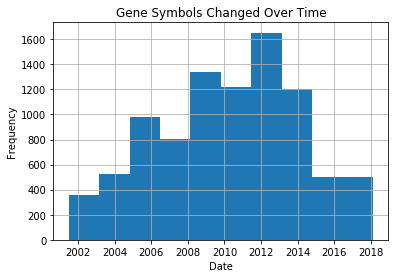
\includegraphics[width=100mm]{figures/gene_symbol_half_life.png}}
    \caption[HGNC Gene Symbol Half Lives]{The frequency by which \ac{HGNC} gene symbols change over time. This figure was generated with the Jupyter notebook available at~\cite{Hoyt2018GeneHalfLife}.}
    \label{fig:gene_symbol_half_life}
\end{figure}

The \ac{MIRIAM}~\cite{Laibe2007} standard was proposed in order to standardize the way named biological entities are referenced in models and databases in order to address the issues with reproducibility arising from the previously described phenomena in natural language as part of the Minimum Information for Biological and Biomedical Investigations~\cite{Taylor2008}.
At its core, \ac{MIRIAM} posits that instead of imprecise names, the bioinformatics community should shift towards using identifiers with five properties: unique (i.e.,\ never assigned to two different entities), perennial (i.e.,\ never changes and is permanent), standards compliant (i.e.\ conform to standards like \ac{URI}, \ac{CURIE}, etc.), free to use, and resolvable (i.e.,\ can be transformed into locations of appropriate online resources).
Note that in the previous section, identifiers were written using the \ac{CURIE} style (e.g., an identifier prefixed with a namespace).
Curiously, the \ac{HGNC} identifier includes a redundant mention of the namespace within the identifier.
Further standardization of redundant \ac{CURIE}s is discussed in Chapter~\ref{ch:bio2bel}.

As Figure~\ref{fig:gene_symbol_half_life} suggests, \ac{HGNC} gene symbols are not perennial and are not \ac{MIRIAM} compliant.
However, even a decade after the proposal of \ac{MIRIAM}, many databases have not yet shifted away from storing and annotating data with \ac{HGNC} gene symbols to using more stable \ac{HGNC} identifiers.

Unfortunately, there has been few or no concerted efforts from authors and publishers to better annotate articles with identifiers for named entities.
Thus, \ac{NER} and entity linking remain relevant as ever, especially due to the increasing volume of literature describing increasingly complex biology across many scales.
